\documentclass[]{report}

\usepackage{fullpage}
\usepackage{graphicx}
\setlength\parindent{0pt}

% Title Page
\title{EVCO Open Assessment}
\author{Y6375144}


\begin{document}
\maketitle

\chapter{Introduction}

\section{Genetic Algorithms}

For some problems it can be difficult to find an optimal solution. This is because the search space grows at a much faster rate (exponentially, for example) than the input space. The Travelling Salesperson problem is a perfect example of this - for a search space with $n$ cities, there are $n!$ paths that the salesperson could take.\\

Evolutionary algorithms do not present a solution to this problem. However, by taking inspiration from biological evolution, they do offer an alternative approach that will often lead to a `good-enough' solution in a much more reasonable number of calculations. \\

Genetic algorithms are a type of evolutionary algorithm that typically represent population members (i.e. candidate solutions) in bitstrings. The population of strings is repeatedly updated through the following process:

\begin{enumerate}
	\item Select - A number of the existing population members are selected to continue through to the next round. Typically these would be the fittest members in the current population.
	\item Crossover - To generate new population members, existing ones are created by crossing two (or more) population members over. See figure \ref{crossoverFigure} for a visual representation.
	\item Mutate - The population is mutated at random. This typically involves passing over every bit in a string, and with a random probability flipping the bit from a 0 to a 1 (or vice versa).
	\item Evaluate - A fitness function is run on each member of the population, giving an indicator of how `good' a solution is.
\end{enumerate}

Genetic algorithms hold much potential, but in order to get the most from them you must carefully choose your representation and parameters. The representation is the bit string typically, but it can also take other forms. There are many parameters that can be fine tuned, such as the number of offspring to breed (at the crossover stage), or the type of crossover to perform.

\begin{figure}[h!]
	\begin{center}
		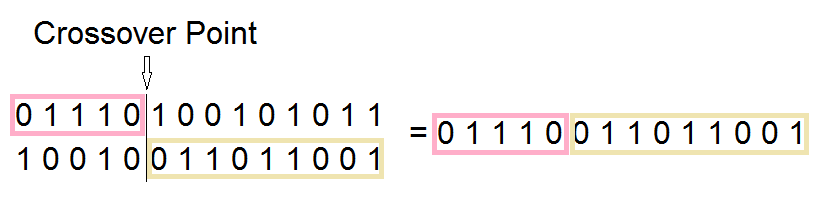
\includegraphics[scale=0.4]{figures/crossover.png}
		\caption{The child is made up of the top row (which represents the first parent) until the crossover point, where it then takes from the bottom row (the second parent).}
		\label{crossoverFigure}
	\end{center}
\end{figure}

\section{The Problem}

Morpion Solitare is a one player game that is typically played on grid paper. To start, a cross shape is drawn in the centre of the page (as shown in figure \ref{morpionSolitare}). On each turn the player must add one cross that creates a line of five crosses either vertically, horizontally or diagonally. The lines may intersect, and in this particular variant the lines may also overlap (it could be argued that this makes the game easier). Figure \ref{morpionSolitare} shows a possible first three moves. Finishing at this stage would give an overall score of 3, as 3 lines of 5 crosses have been formed.\\

\begin{figure}
	\centering
	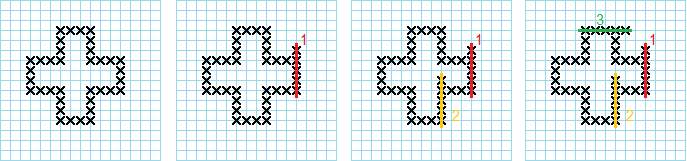
\includegraphics[width=\textwidth]{figures/combinedthreemoves.png}
	\caption{The initial state of the game on the left, and from left to right the first three moves are shown. The lines don't have to be numbered, but for clarity they are here.}
	\label{morpionSolitare}
\end{figure}

In this report I will detail my investigation into obtaining a high score through the use of a genetic algorithm. Working out the fitness of a population would be a tedious process if I have to take each population member and draw out its game from scratch. Thankfully that is not necessary as I have been provided with a computerised version of the game that is slightly faster.\\

When designing my genetic algorithm I will have to consider the format that the digital version takes its input by. The program represents positions on the grid by their $(x, y)$ co-ordinate positions, where $(0, 0)$ is the bottom left of the grid. For each move, four parameters must be passed into the program in the format $x_1 y_1 x_2 y_2$, where $(x_1, y_1)$ is the position of one end of the line to draw, and $(x_2, y_2)$ is the other end of that line. For the game shown in figure \ref{morpionSolitare}, the input would be:

\begin{verbatim}
	linuxMsolitare.exe 12 11 12 7 9 9 9 4 6 13 10 13
\end{verbatim}

The program accepts a maximum of 2000 inputs, or 500 moves. Given that the current best known solution is 178 \cite{morpionRecord}, this is unlikely going to be a problem. One potential problem is that to evaluate a population of size $n$, the application will need to be called $n$ times. Even with a decent processor, this could be a slow task for any sizeable population. Also, if a representation is chosen that doesn't directly map to the program's inputs is chosen, then each population member's representation will have to be converted to the correct format before the program can even be called. Again, this could be time consuming, but solutions to these problems will be considered in the next section.


\chapter{The Solution}

\section{Representation}

The standard genotype in a genetic algorithm is a bit-string. Studies have shown that in a lot of cases the algorithm will perform better when a bit string is used \cite{something}, although other studies suggest that this is not necessarily the case \cite{somethingElse}.\\

I will now discuss possible representations, and then explain my choice of representation.

\subsection{Gray Code Bit-string}

Binary bit-strings are not ideal for a genetic algorithm as a single bit flip during the mutation stage can cause the number to change a lot. Consider the bit string $10010110$ that represents the 8 bit unsigned integer 150. During mutation, if just the first bit is flipped, the string becomes $00010110$ and now represents 22. If the search space is a 256x256 grid, and that integer represents one co-ordinate, then 150 to 22 is a large jump. It would be more useful if the co-ordinate changed by just a small amount. If we wanted to change to 149 ($10010101$), two bit flips are required. \\

One solution to this is to use Gray code. This is a bit-string where each consecutive value differs by only one bit. In Gray code, $11011101$ represents 150, and $11011111$ represents 149. That's just a single bit flip, making Gray code ideal for genetic algorithms. \\

There are now a few possible options for how Gray code could be used to represent an individual move, and then a series of moves. The first option is to represent the co-ordinates as they are passed into the program in Gray code (remember that a move is passed in to the program as $x_1 y_1 x_2 y_2$). The grid 40x40, so ($\log _2 40 = 5.32$) 6 bits would be required to represent each co-ordinate. Each move would use 24 bits, and if the maximum number of moves is played each time (500), then 12000 bits or 1500 bytes will be required for each population member. If we have a population size of 5000, then the total required space will be 7.15MB.  \\

The second option is to store each move as a combination of (co-ordinate, direction), where co-ordinate is the new cross to draw on the board, and direction is the direction of the line. So ((20, 20), left) would mean draw a cross at position (20, 20), and draw left. This would then be translated into the program's input format $x_1 y_1 x_2 y_2$ to be 20 20 15 20. Again, 6 bits would be required to represent each co-ordinate. As there are 8 possible directions, ($log_2 8$) 3 bits are required to represent the direction that the line should be drawn in. Therefore each move would use 15 bits, giving a maximum of 7500 bits or 938 bytes for each population member. With a population size of 5000, the total required space will be 4.47MB. This is a good saving on the last representation described. However, computers nowadays have a lot of memory, and the difference between 4.5MB and 7.2MB is tiny relative to the standard 4GB of memory that a low-end computer has. There is also the overhead to consider when the representation has to be converted into program input. The first described representation would be the fairly simple task of converting Gray code to an integer. With this representation, the overhead would be slightly higher, as the start position and direction would need to be considered in order to calculate the program input. \\

The third and final possible representation that uses Gray code does not use the co-ordinate system as it has been previously described. Starting at the bottom left and moving right, each position will be assigned a single integer. When the end of the row is reached, the above position will be numbered, and then on that row moving left the positions will be numbered. See Figure \ref{alternativePositioning} for a visual explanation. As the grid is 40x40, 1600 positions will be numbered. Describing a move will be done as above, with (postion, line direction). The amount of storage space required will be ($log_2 1600$) 11 bits for the position, and 3 again for the direction. This uses 14 bits per move in total, and sticking with the already used example of 500 moves per population member and 5000 population members will use a total of 4.2MB. A slight saving on the previous representation, but again the overhead increases as we now also have to convert between the new position representation as well as the direction representation. Another disadvantage that comes with this representation is that it is more difficult during the mutation stage to move a move in a particular direction. If you wanted to mutate the population member by changing one of its moves to start two rows above, you have to perform a relatively complex calculation in order to work out the number assigned to the position two rows above. With the above two representations it is easy to convert the Gray code to an integer, add 2 to the y co-ordinate, and then convert back to Gray code. Even better (although not necessarily easier to code) would be to perform the arithmetic in Gray code. \\

\begin{figure}
	\centering
	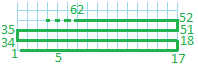
\includegraphics{figures/alternativeRepresentation.png}
	\caption{An alternative co-ordinate representation that starts at the bottom left of the grid numbering each position as shown.}
	\label{alternativePositioning}
\end{figure}

\subsection{Integer Representation}

The natural input to the program is a set of integers. Using any other representation internally requires that a conversion takes places before the fitness of the population can be calculated. Because of this, it's worth weighing up the pro's and con's of using an integer representation.\\

To help understand a reason why an integer representation may be worth considering, I go back to looking at the use binary or Gray code. Consider the move 20 20 24 24 that draws a diagonal line from the centre of the grid to the position (24, 24). If we were using a binary representation with 6 bits for each co-ordinate, the move would look like:

\begin{center}
\begin{verbatim}
	010100 010100 01100 011000
\end{verbatim}
\end{center}

We then perform a mutation operator on the representation that has a 10\% probability of flipping each bit that it comes across. It outputs the following:

\begin{verbatim}
	110100 010101 01100 011100
\end{verbatim}

This is the same as 56 21 24 28, an invalid move because the board is limited to 40x40, and also because no the co-ordinates don't represent a line that is 5 positions long. \\

Using an integer representation then the mutation operator would know what changes could be made to a group of integers that would still be valid, and only perform these. For example, with 20 20 24 24, it might decide to shift down by 2 rows, and so it would subtract 2 from the y co-ordinates. Of course there is no reason why this can't be done with a binary representation - using binary arithmetic 000010 could be subtracted from each x co-ordinate, but using binary provides no advantage over using an integer representation, but does include the disadvantage that when used in the `pure' genetic algorithm sense (i.e. flipping bits at random), then there is a high probability of creating an invalid move. Of course this is counteracted by using Gray code, but now we consider crossover. \\

To confirm that using an integer representation instead of Gray code doesn't disadvantage the algorithm, we must also analyse the effect on crossover. Consider the below samples of two population members in binary / Gray code (for this section the point holds for both representations):

\begin{verbatim}
	... 011111 011111 011111 0100011 001100 000001 001000 000001 ...
	... 000000 000001 000000 0000101 101000 000110 100100 000010 ...
\end{verbatim}

The top one describes the move 31 31 31 35 12 1 8 1, and the bottom describes 0 1 0 5 40 6 36 2. With a naive crossover algorithm, any point in the two binary strings could be chosen to crossover. The above samples each have 48 bits, so let's randomly choose to swap at bit 37. The two new population members are now:

\begin{verbatim}
	... 011111 011111 011111 0100011 001100 000001 000100 000010 ...
	... 000000 000001 000000 0000101 101000 000110 101000 000001 ...
\end{verbatim}

The top member now represents 31 31 31 35 12 1 4 2, and the bottom 0 1 0 5 40 6 40 1. The second move in each member has been made invalid, reducing the fitness of the member. The chances of performing a crossover and increasing the fitness around the crossover point with a binary representation is therefore low. However, it could still be the case that ultimately the fitness of the member is increased as the moves before the crossover point combined with the moves after the crossover point could together improve the overall fitness. \\

It is not hard to imagine a situation where the crossover produced a number that is greater than 40, thus rendering the move invalid. To counter these problems we could improve the crossover algorithm to only crossover after whole numbers (i.e. where bit position MOD 6 = 0). If this approach is to taken though, we may as well be using integers because we will only be crossing over in the same position as if we were using integers. \\

\subsection{Conclusion}

Because I do not believe that using a binary/Gray code representation will provide an advantage, and because an integer representation will be easier to debug and quickly analyse, I have decided to use an integer representation. In the Gray Code Bit-string section I discussed the different representations that could be used, such as giving every position on the board a single number, and then following that by a direction. The same could be done with an integer representation, but I have dismissed this for the same reasons as before: the overhead associated with converting between two formats does not appear to outweigh the small advantage of using less memory. \\

\section{Selection}
Now that a representation has been decided on, each stage of the genetic algorithm must be decided on. The first of these is selection. With a population in whose members we know the individual fitness of, we must decide which of the members to take through to the next generation, and which should be discarded to be replaced by crossed over and mutated population members.

\subsection{Highest Ranking}

The Highest Ranking selection algorithm is very simple. The population members are sorted in order of fitness, and then a fraction of the top members are selected to continue to the next round. \\

At first glance this sounds like an ideal solution. To understand why this is not necessarily the case, imagine if the population members were dogs. While choosing which dogs to breed to create a new generation of dogs, we only choose the dogs that are the best looking. One particular ugly dog is not chosen to be bred, but what we didn't know is that if it had been bred with some other dog then it would produce very attractive offspring. This is an extreme example, but the underlying point is that just because the fitness of a population member is not currently high does not necessarily mean that it won't be useful in the future.\\

\begin{figure}
	\centering
	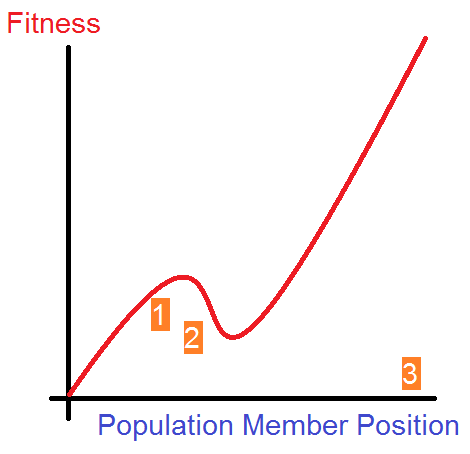
\includegraphics[scale=0.4]{figures/highestRanking.png}
	\caption{A simplified example of population members and their fitness}
	\label{highestRankingProblem}
\end{figure}

Figure \ref{highestRankingProblem} gives a visual example of this. Each orange box is a population member, the $x$-axis is the current position of the population member in a search space, and the $y$-axis is the fitness measurement. Current population members 1 and 2 would be chosen over 3 in the highest ranking algorithm. What we don't know is that if 3 had been selected and crossed with another population member then it could easily have had a higher fitness that 1 or 2 currently have. By selecting 1 and 2 we have got stuck in a local maxima.

\subsection{Roulette Wheel}

In order to overcome the problems with highest ranking selection we must allow for low fitness population members to be included, but we also want to include mainly high fitness population members. A good way of doing this is to select population members with a probability that is proportional to their fitness. So if the sum of fitness across the whole population is 360, and the fittest population member has a fitness of 90, then there is a $\frac{90}{360}$ or $\frac{1}{4}$ chance of the population member being included in the next generation.\\

Figure \ref{rouletteWheel} gives a visual representation of this: the whole area of the wheel represents the summed fitness of the population, and each segment is the proportional fitness of a population member. In the left-hand example, the yellow population member has the highest fitness, and is therefore the most likely to be chosen to continue to the next generation. The green population member has the lowest fitness, and only has a slim chance of being carried through to the next generation. This does not completely fix Highest Ranking's problem that was demonstrated with Figure \ref{highestRankingProblem}, but it is an improvement because it at least gives population member 3 a chance of roulette wheelbeing carried into the next generation.\\

\begin{figure}
	\centering
	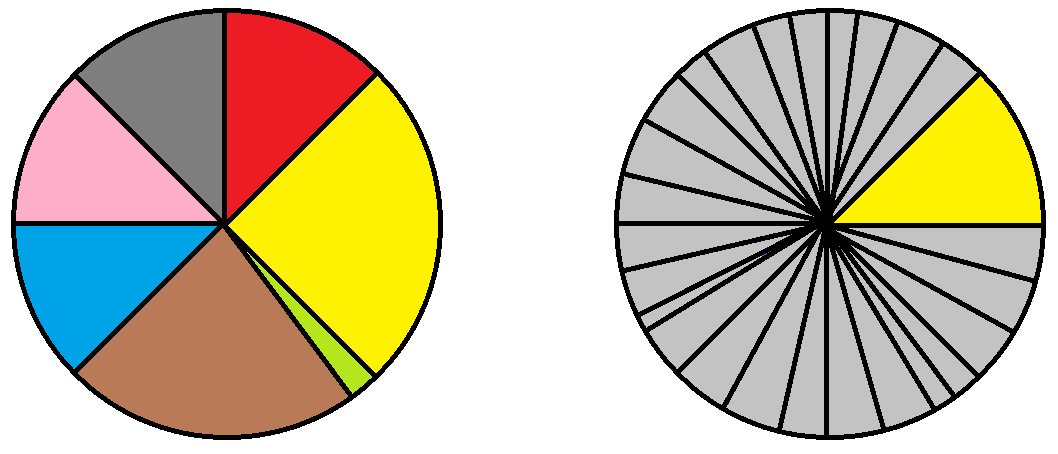
\includegraphics[scale=0.4]{figures/rouletteWheel.png}
	\caption{Two visual representations of roulette wheel selection}
	\label{rouletteWheel}
\end{figure}

Looking again at Figure \ref{rouletteWheel}, but this time the right-hand wheel, we can see the problem with roulette wheel selection. If there is one population member that is significantly fitter than the group average, the chances of it being chosen aren't high enough. For example, if we want to choose a third of the population to take to the new generation, there is a good chance that strongest population member (yellow) will not be chosen.

\subsubsection*{Elitism}

A fix for this problem is to introduce elitism. This is when the fittest population members are immediately chosen for the next generation, and then roulette selection is performed. This is not perfect because if you have one population member with fitness 90, and then twenty members with fitness 89, and six hundred members with an average fitness of 10, then you still only guarantee that the single 90 fitness population member will be carried to the next generation. We could of course say that the two top fitness ratings will be considered, but again the problem could be a 90 fitness member, an 89 fitness member, nineteen 88 fitness rated members and six hundred members with an average fitness of 10. Elitism is unfortunately more of a workaround than a fix.

% TODO: If there's space, discuss and dismiss other methods of selection

\subsection{Conclusion}

I will implement all of the above selection methods, and test each to determine which results in the best final result.

\section{Crossover}

Crossover has fewer decisions to make than selection. To create a new population member we must select two population members (that were selected during the selection stage), look at their list of moves, and decide which moves from each population member to use for the new population member. The decision to make is in when to use the first parent's data, and when to use the second parent's data. (By data I mean the genotype.)\\

In the simplest solution, a random $n$ would be picked that is less than the smallest parent's data. The first parent's data would be copied until position $n$, and then from there the second parent's data from $n$ until the end would be copied. In figure \ref{crossoverFigure}, the value $n$ is the crossover point. \\

The immediate problem that can arise from this with the chosen representation is that is if a crossover point is chosen that isn't between two moves (where a move is a set of 4 integers), then the new move that is created on that point has a high chance of being invalid. How much of a problem this is will be discussed in the results section after I have tried and compared the completely random approach, and the approach that continues to randomly select numbers until one which is between two moves. \\

Another consideration is how many crossover points should be used. The simple approach uses a single crossover point, but when the data size of a population member can be up to 2000 integers, better results may be obtained by crossing in multiple places. These places could be completely random, or selected such that they are between moves. How many positions is optimal will be discussed in the results section. \\

The final consideration is how many parents should be used. Up to this point only two parents has been considered, but there is no reason why three, four, five or even more parents could be used. Of course this would require multiple crossover points, and each crossover point could  Again this is another question that will be answered in the results section.

\section{Mutation}

After selection and crossover, we have a new generation. A small amount of mutation within the new generation allows new solutions to be found that are not currently within the population. Mutation ensures that convergence at a local maxima won't prevent the population from moving to a higher fitness. It may take many generations, but with a decent mutation operator eventually the local maxima will be escaped and fitter members can be generated.\\

The naive mutation operator will move across every population member, and every piece of data in the population member (in this case the list of integers), and with a fixed probability change the data item to some other random data. With my chosen representation each integer changed to some other integer between 0 and 40 with a small probability.

\chapter{The Results}

\section{Conclusion}

\bibliography{bibliography}

\end{document}          
